\chapter{Pile head rotation as function of embedded pile length}\label{sec_3}


In Figure ~\ref{pilehead_vs_length} the pile head rotation is plotted as function of the embedded pile length. The figure provides information of the robustness present in the design and hence provides input in the selection of embedded pile length. With the selected embedded pile length, the design is far from the steep part of the curve, therefore indicating a robust design.

\begin{figure}[!htbp]
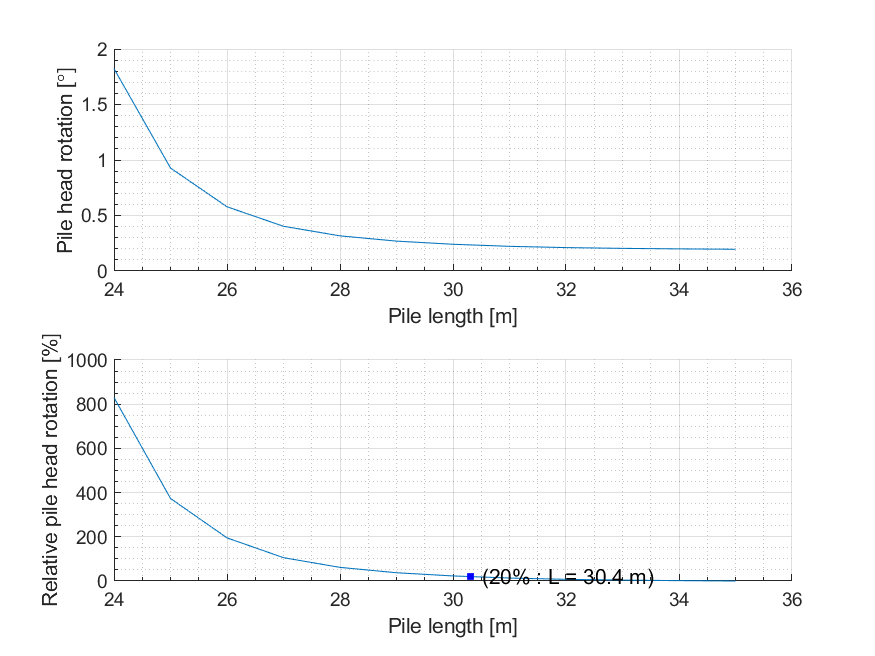
\includegraphics[width=0.9\textwidth]{AppendixGenerationFiles/ProjectLocation/pilehead_vs_length.png}
\caption{Pile head rotation against pile embedded length for unfactored ULS loading at WTG {\ID_location}. Characteristic soil properties adopted and with the effect of cyclic degradation considered.}
\label{pilehead_vs_length}\end{figure}
